
\section{Introduction}
\subsection{Context}
\begin{frame}
  \frametitle{Context: Sciences usign neutrons}
  Thermal and cold neutrons are useful tools to probe matter
  \begin{itemize}
    \item Neutral particle, high penetration and low EM interaction
    \item Wave–particle duality, important wavelength range
    \item Various techniques: diffraction, reflectometry, spectrometry
  \end{itemize}
  \begin{columns}
    \begin{column}{0.65\textwidth}
      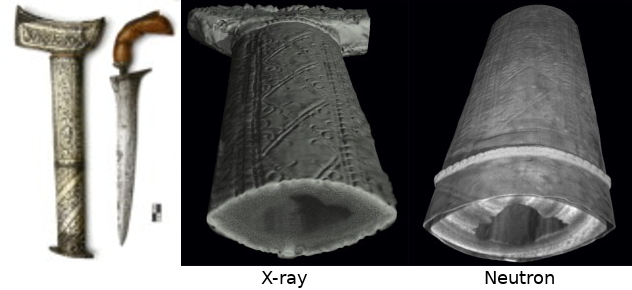
\includegraphics[width=\textwidth]{01_Neutron/fig/fig000_Dague2.png}
    \end{column}
    \begin{column}{0.3\textwidth}
      \begin{block}{Example: dagger cover}
        \begin{itemize}
          \item Internal structures
          \item Synergy with X-rays
        \end{itemize}

      \end{block}
    \end{column}
  \end{columns}
  \begin{block}{Application in various field}
    Archeology, Geosciences, Life Science, Chemistry
  \end{block}
\end{frame}

\begin{frame}
  \frametitle{State of neutron sources}
  Producing an intense neutron flux is not a trivial task.
  Current intense sources are mainly based on two different methods:
  \begin{columns}[T]
    \begin{column}{0.45\textwidth}
      \begin{block}{Fission reactor}
        \begin{itemize}
          \item Uses fission reaction.
          \item $_{92}^{235}U + n \rightarrow X + Y + k \times n$
          \item $k\approx2.45$ per reaction.
          \item Continuous flux (most of time).
        \end{itemize}
      \end{block}
      \vfill
    \end{column}
    \begin{column}{0.45\textwidth}
      \begin{block}{Spallation source}
        \begin{itemize}
          \item Uses particle accelerator
          \item Impact of heavy particle on dense target.
          \item Around $20 \sim 40$ per incident particle.
          %\item Expensive method.
        \end{itemize}
      \end{block}
      \vfill
    \end{column}
  \end{columns}

  %Spallation sources benefit of the improvement of accelerator technology over years and become more and more popular.
\end{frame}

\subsection{State of neutron sources}
\begin{frame}
  \frametitle{State of neutron sources}
  From "Neutron scattering facilities in Europe" report by ESFRI:
  \begin{columns}
    \begin{column}{0.50\textwidth}
      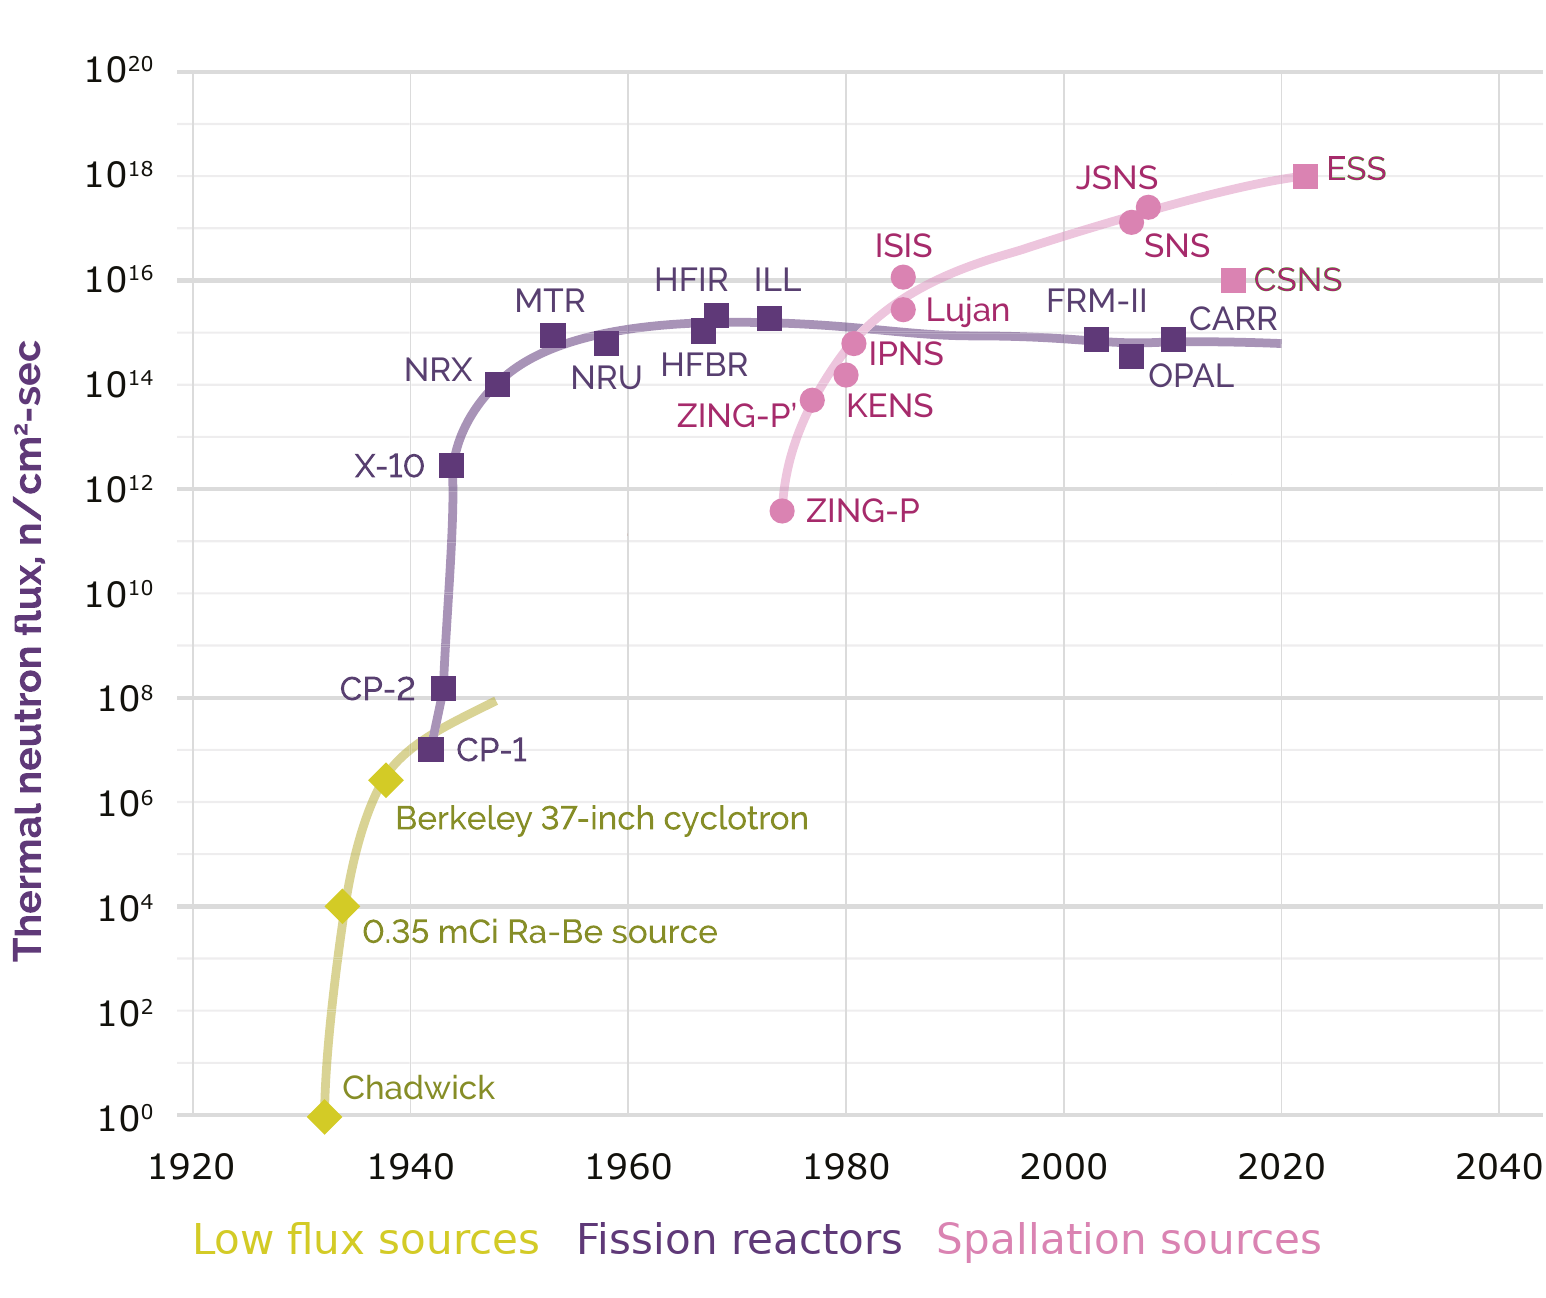
\includegraphics[width=\textwidth]{01_Neutron/fig/fig000_NeutronSources_a2}
    \end{column}
    \begin{column}{0.50\textwidth}
      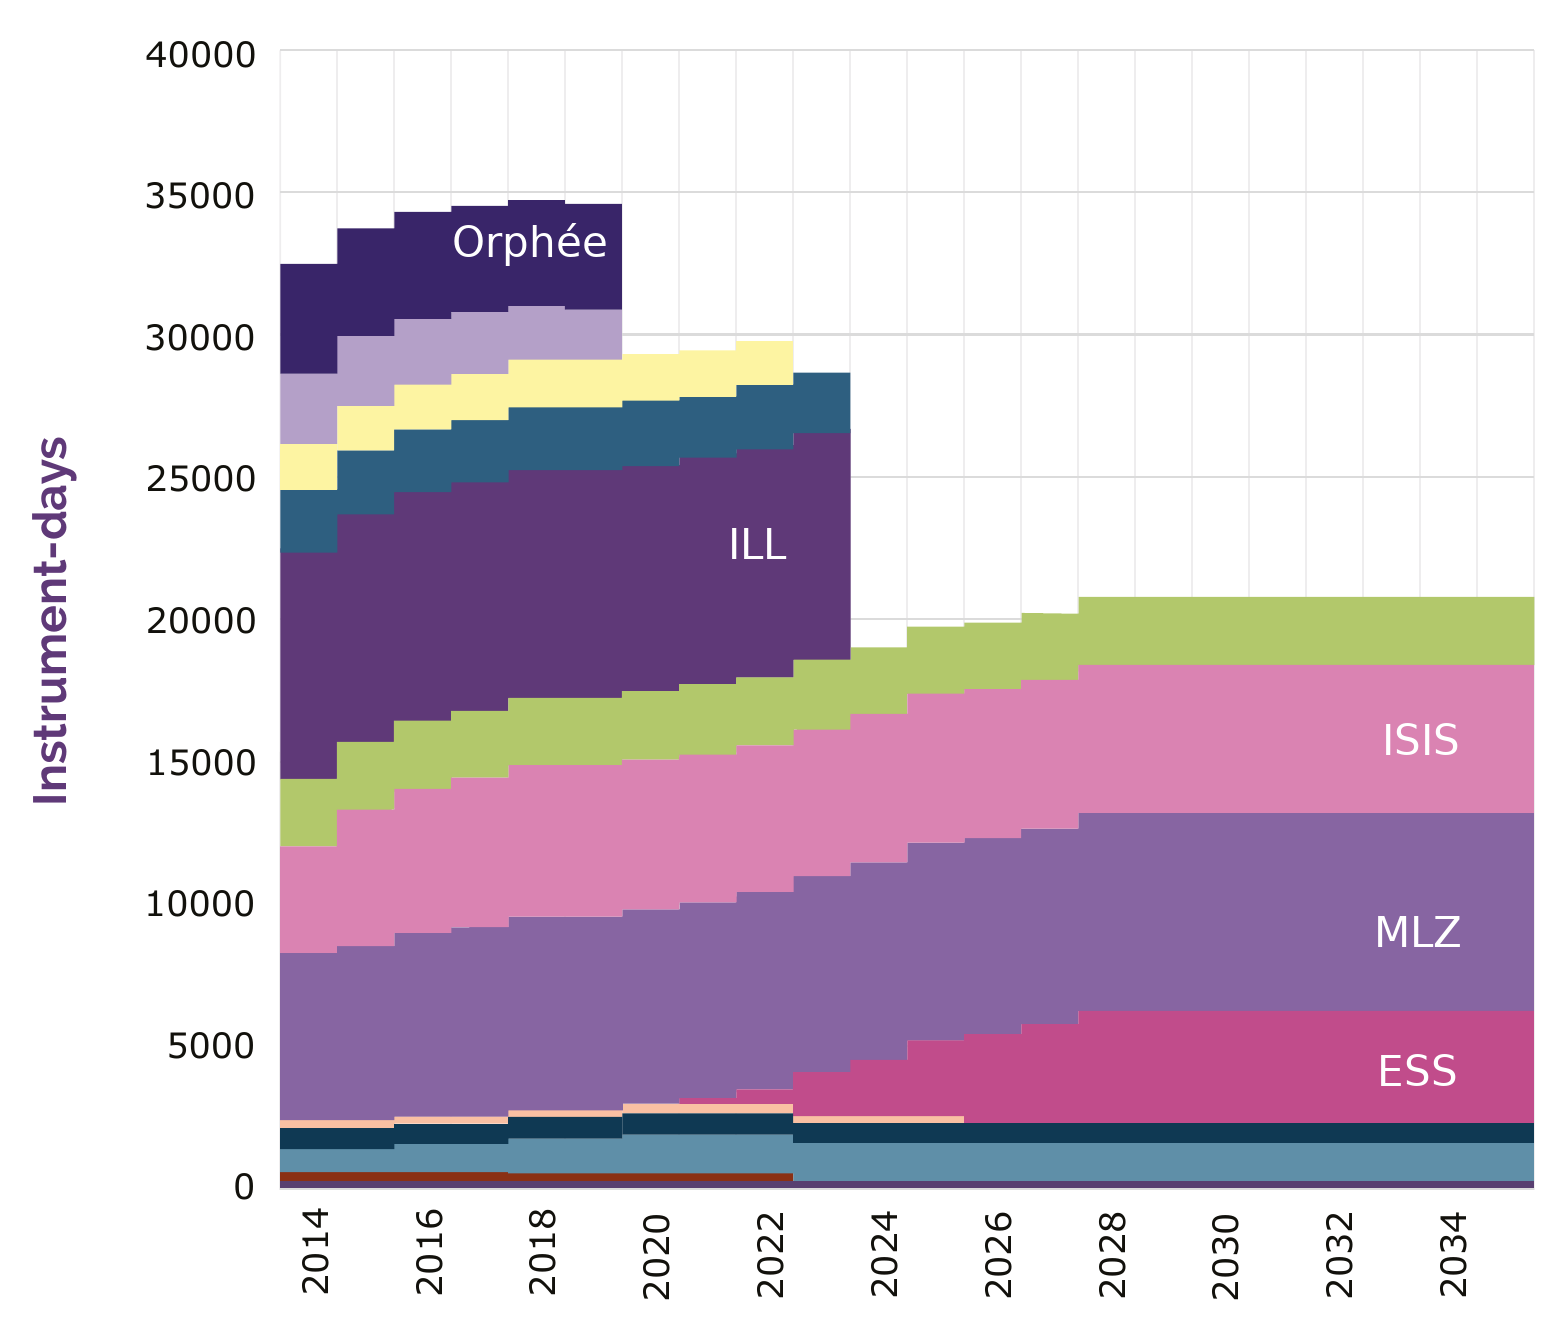
\includegraphics[width=\textwidth]{01_Neutron/fig/fig000_NeutronSources_b2}
    \end{column}
  \end{columns}
  \begin{alertblock}{The future does not look great in Europe}
    \begin{itemize}
      \item Many old fission reactor $\rightarrow$ end of life within the next decade.
      \item Only 1 major spallation source $\rightarrow$ 1$^{st}$ Gen source, 35 years old.
    \end{itemize}
    A renew is necessary in Europe, built upon a new flagship source.
  \end{alertblock}
\end{frame}

\begin{frame}[t]
  \frametitle{European Spallation Source}
  \centering
  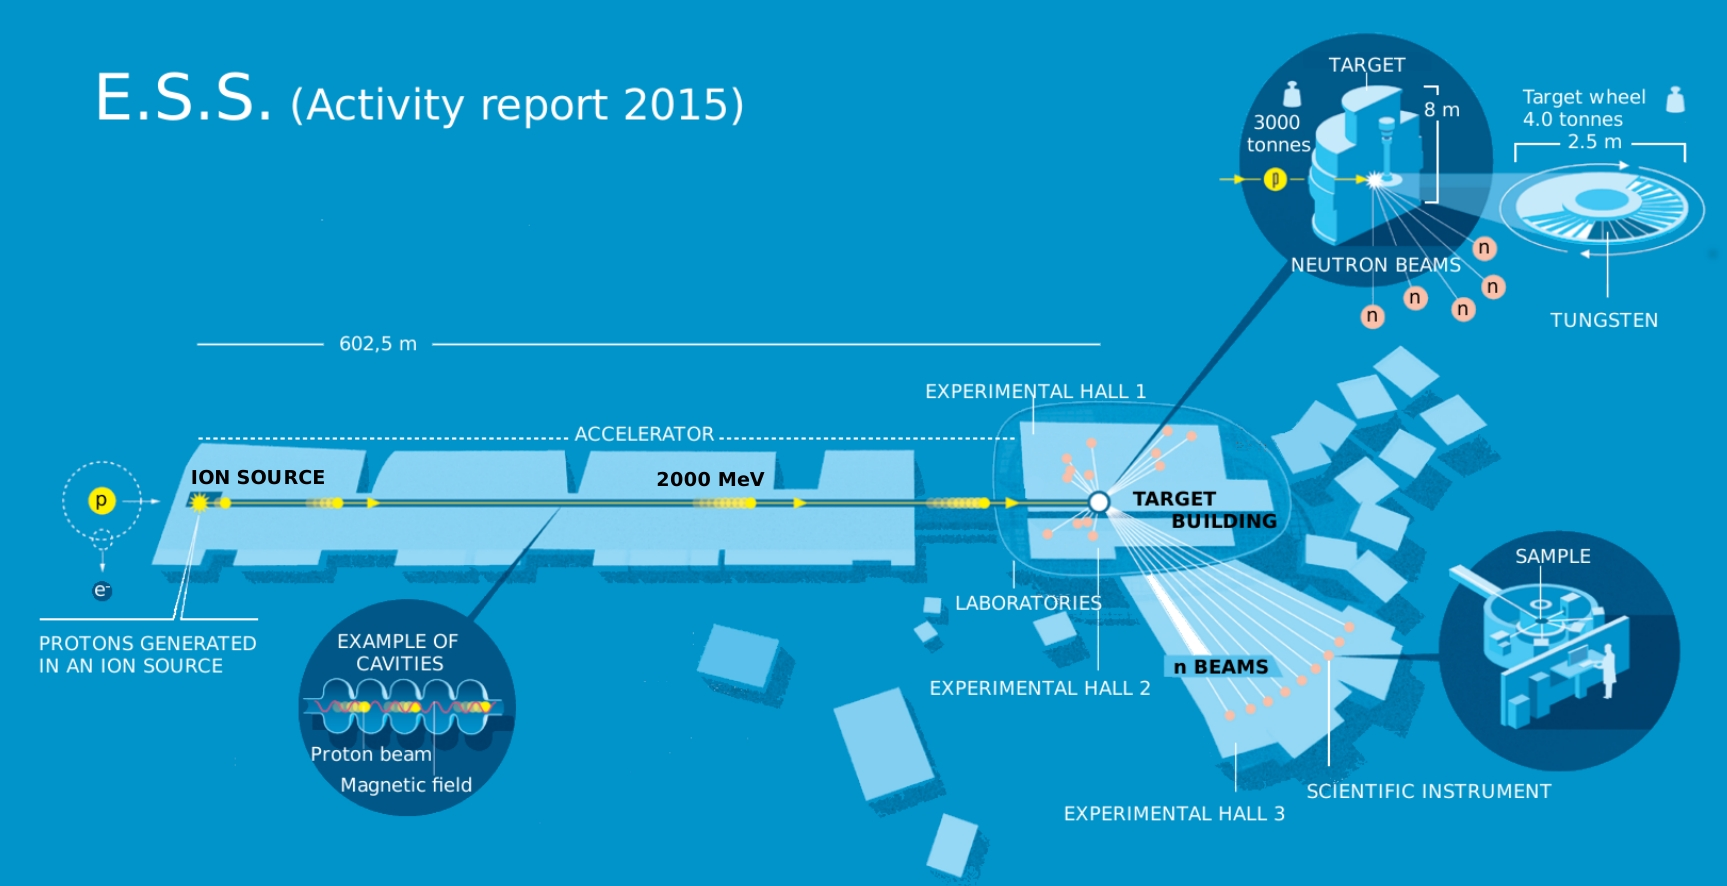
\includegraphics[width=1.\textwidth]{01_Neutron/fig/fig000_ESS_com}
  Proton accelerator + Tungsten target $\implies$ Neutrons + Instruments
\end{frame}

\subsection{European Spallation Source}
\begin{frame}
  \frametitle{European Spallation Source}
  ESS will be the most powerful neutron source.
  Based on a 2 GeV proton accelerator and a tungsten target
  \begin{columns}
    \begin{column}{0.35\textwidth}
      \begin{block}{Key points}
        \begin{itemize}
          \item[2014] Ground breacking
          \item[2021] First protons on target
          \item[2023] Beginning of user program
          \item 15 instruments
          \item Total cost: 1.8 B€
        \end{itemize}
      \end{block}
    \end{column}
    \begin{column}{0.60\textwidth}
      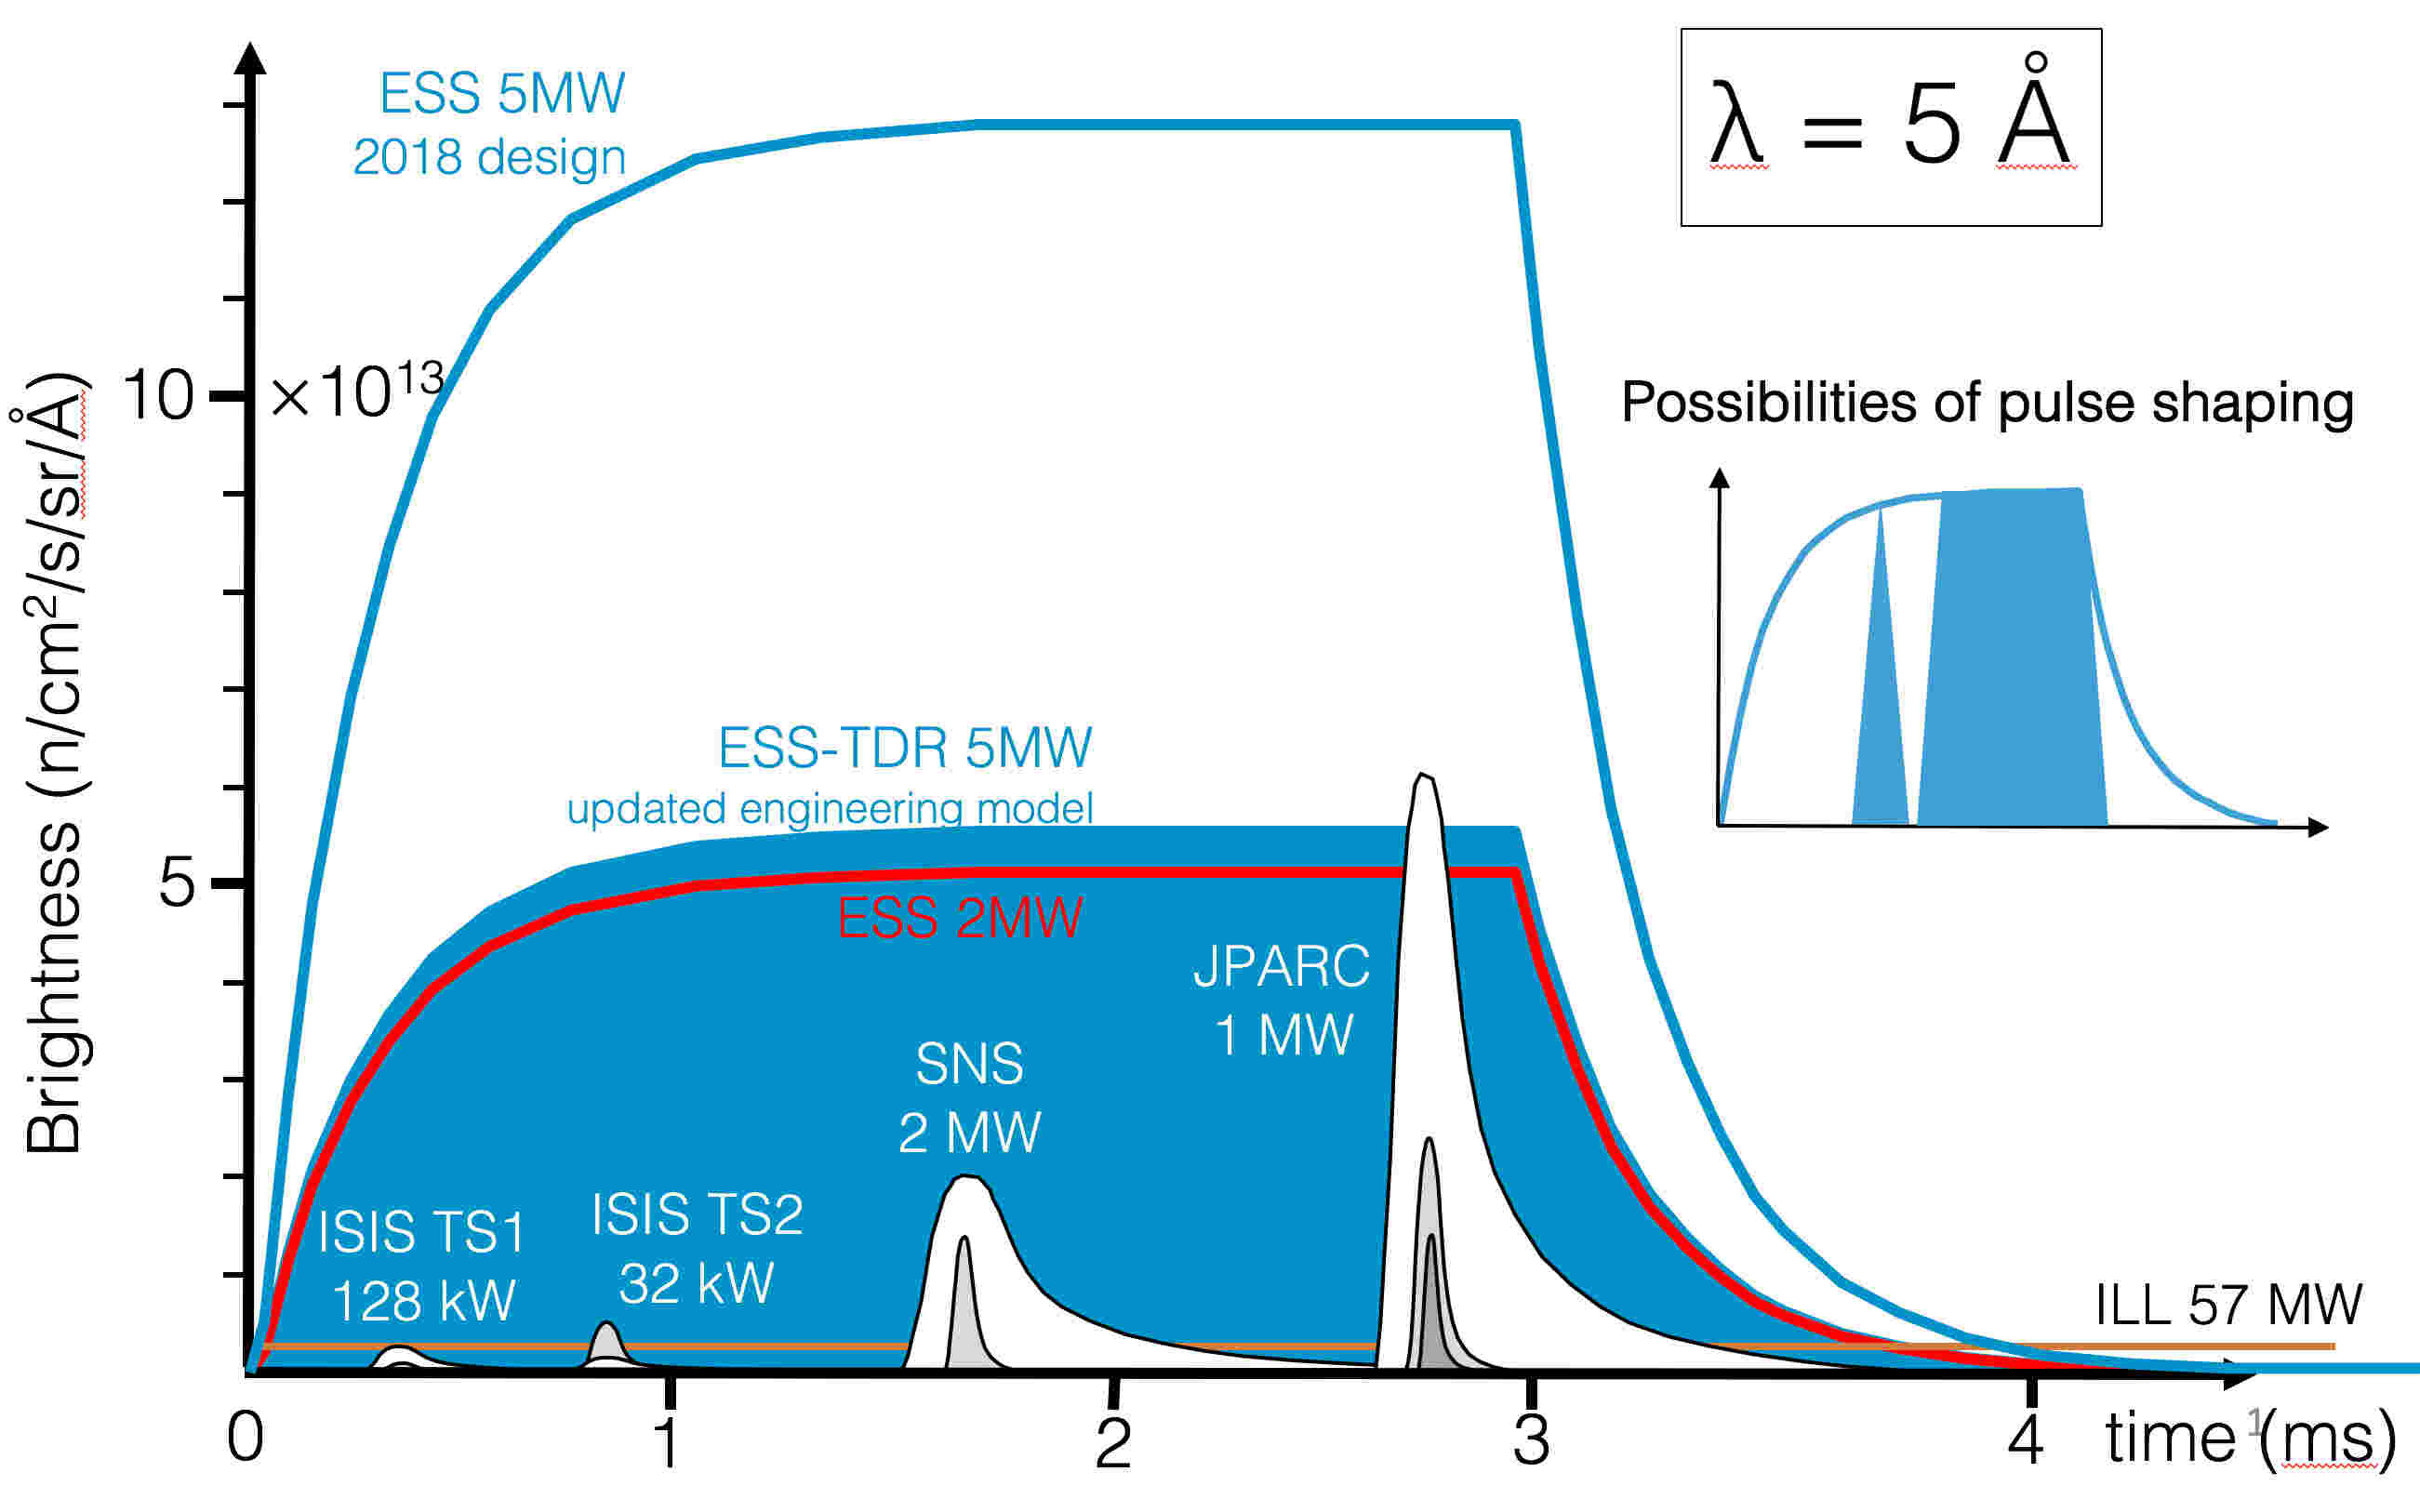
\includegraphics[width=\textwidth]{01_Neutron/fig/fig000_ESS_pulse2.jpeg}
    \end{column}
  \end{columns}
  \begin{block}{Why ESS is different?}
    Long pulses \& high intensity $\implies$ more protons on target $\implies$ more neutrons

    Single shoot pulse, no use of accumulator ring $\implies$ the accelerator must be enough powerful.
  \end{block}
\end{frame}

\subsection{The ESS accelerator}
\begin{frame}
  \frametitle{The ESS accelerator}
  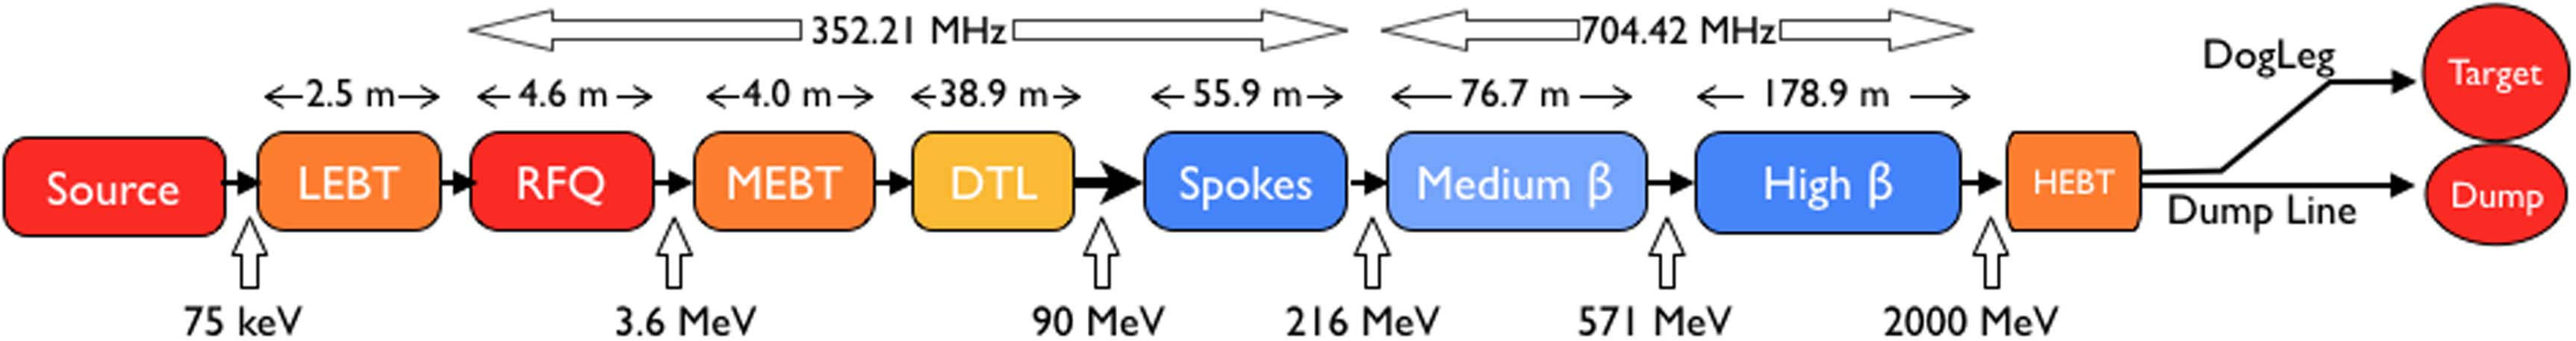
\includegraphics[width=\textwidth]{01_Neutron/fig/fig000_ESS_acc}
  \vfill
  \begin{columns}
    \begin{column}{0.45\textwidth}
      The accelerator itself is a big challenge:
      \begin{itemize}
        \item $600\,\mathrm{m}$ long with $356\,\mathrm{m}$ of acceleration
        \item Heavy use of SC cavities (95.5\% of acceleration)
      \end{itemize}
      \begin{block}{ESS activities at IRFU}
        \begin{itemize}
          \item RFQ
          \item Cryomodules
          \item Diagnostics
          \item Control System
        \end{itemize}
      \end{block}
    \end{column}
    \begin{column}{0.50\textwidth}
      \begin{tabularx}{\linewidth}{XX}
        \toprule
        Characteristic & Value                                 \\
        \midrule
        Energy         & $2\,\mathrm{GeV}$                     \\
        Current        & $62.5\,\mathrm{mA}$                   \\
        Duration       & $2.86\,\mathrm{ms}$                   \\
        Rep. rate      & $14\,\mathrm{Hz}$                     \\
        Duty cycle     & $4\,\mathrm{\%}$                      \\
        Power (peak)   & $5\,\mathrm{MW}$ ($125\,\mathrm{MW}$) \\
        RF             & $352.21\,\mathrm{MHz}$                \\
                       & $704.42\,\mathrm{MHz}$                \\
        \bottomrule
      \end{tabularx}
    \end{column}
  \end{columns}
\end{frame}